\documentclass[11pt]{article}
\usepackage[margin=1in]{geometry}
\usepackage{booktabs}
\usepackage{amsmath}
\usepackage{graphicx}
\usepackage{natbib}
\usepackage{hyperref}
\usepackage{float}

\title{Longitudinal CEA Trajectories and Disease Progression Prediction in Colorectal Cancer}
\author{Yanan Fang}
\date{April 4, 2026}

\begin{document}
\maketitle

\begin{abstract}
\noindent
Carcinoembryonic antigen (CEA) is the standard surveillance biomarker for colorectal cancer, but routine practice relies on static thresholds that ignore the temporal dynamics of biomarker change. Using the MSK-CHORD 2024 release, we ask whether longitudinal CEA trajectory features improve 180-day disease progression prediction beyond standard clinical variables, and whether somatic mutation status adds further predictive value. We assemble a landmark dataset of 68{,}272 CEA-anchored prediction time points from 3{,}950 colorectal patients and fit three models: a clinical-only generalized linear mixed model (Model~0), a clinical model augmented with the current $\log(\text{CEA})$, the 90-day slope, and the within-patient coefficient of variation (Model~A), and a LASSO logistic regression that adds tumor mutational burden and indicators for the ten most recurrently mutated CRC genes (Model~B). On a patient-level held-out test set, adding CEA trajectory features raises the AUC from 0.647 to 0.703 (DeLong $p = 3.6 \times 10^{-10}$); the genomic LASSO does not move the AUC further (0.703 on the shared subset, $p = 0.98$) but modestly improves the calibration slope. Split-conformal prediction sets achieve 90.1\% empirical coverage with 34.7\% singleton informativeness, concentrated at the extremes of predicted risk. The results indicate that the shape of recent CEA trajectories carries signal that single-point thresholds miss, while gene-level mutations are largely redundant with the clinical and CEA features at the discrimination level.
\end{abstract}

\section{Introduction}

Carcinoembryonic antigen (CEA) is the most widely used serum biomarker for colorectal cancer (CRC) surveillance. In current clinical practice, CEA monitoring typically relies on static thresholds (e.g., $>5$~ng/mL) to flag potential disease progression. However, single-point cutoffs have limited sensitivity and fail to capture the temporal dynamics of biomarker change that may precede radiographic evidence of progression.

Longitudinal CEA trajectory features---such as the rate of change (slope) and within-patient variability (coefficient of variation)---may encode disease dynamics missed by static values. A rising CEA slope, for instance, could reflect accelerating tumor growth before a formal progression assessment, while high CEA variability might indicate an unstable disease state. Extracting these features within a \emph{landmark prediction framework} enables dynamic risk assessment at each clinical visit, using only information recorded up to the landmark day and thereby minimizing information leakage from future data.

The question we therefore ask of the MSK-CHORD colorectal cohort is whether longitudinal CEA trajectory features improve 180-day disease progression prediction beyond standard clinical variables. Our working hypothesis is that a rising CEA slope and higher within-patient variability are associated with increased short-term progression risk, so that a mixed-effects model that incorporates these features should discriminate better than a clinical-only baseline.

We employ three complementary approaches: (1) a clinical-only generalized linear mixed model (GLMM) as a baseline (Model~0), (2) a GLMM augmented with CEA trajectory features to quantify their incremental value (Model~A), and (3) a LASSO logistic regression incorporating genomic covariates to assess whether gene-level mutations add further predictive power (Model~B). We additionally apply split-conformal prediction to construct finite-sample valid prediction sets for the binary progression outcome.

\section{Variables Used and Data Cleaning}

The analysis integrates seven datasets from the MSK-CHORD 2024 release: patient-level clinical data, sample-level metadata, CEA laboratory results, progression assessments, diagnosis timeline records, treatment records, and somatic mutation calls (see Supplementary Table~S1 for details).

Cohort construction proceeded as follows. Samples were restricted to patients with cancer type ``Colorectal Cancer'' ($n = 5{,}543$). For patients with multiple tumor samples, the sample with the highest sequencing coverage was retained. Diagnosis anchoring used CRC-specific primary diagnosis records identified via ICD topography codes (C18--C21) and anatomical keywords (colon, rectum, cecum, sigmoid). One patient without any primary diagnosis record was excluded. Gene mutation indicators were constructed for the 10 most recurrently mutated genes in this CRC cohort: \textit{APC}, \textit{TP53}, \textit{KRAS}, \textit{PIK3CA}, \textit{FBXW7}, \textit{SMAD4}, \textit{TCF7L2}, \textit{ARID1A}, \textit{SOX9}, and \textit{BRAF}.

CEA measurements were filtered to non-negative, non-missing values and converted to the log scale ($\log(\text{CEA} + 0.1)$). Patients with fewer than three CEA measurements were excluded, leaving 4,996 patients with 104,496 CEA records.

A complete enumeration of analytic variables, their source files, and coding rules is provided in Supplementary Table~S1.

\subsection*{Landmark Dataset Construction}

In the landmark prediction framework, each CEA measurement from the third onward serves as a potential prediction time point. We let the landmark time $t$ denote the number of days from the patient's CRC primary diagnosis (the \texttt{START\_DATE} of the primary-diagnosis record in \texttt{data\_timeline\_diagnosis}, rescaled so that $t = 0$ on the day of diagnosis) to the day of the CEA measurement. Defined this way, $t$ is a positive integer in days that varies from landmark to landmark within the same patient and is zero only at the day of diagnosis, not at the first CEA draw. All time-varying covariates---log CEA, the 90-day slope, the coefficient of variation, treatment status, and time since diagnosis---are constructed on this diagnosis-anchored scale and use only information available up to $t$.

At each landmark we record four features. The current CEA value enters as $\log(\text{CEA}(t) + 0.1)$. The 90-day slope is the ordinary least squares coefficient of $\log(\text{CEA})$ regressed on time using every measurement falling within $[t-90, t]$; at least two measurements in this window are required, and landmarks without a computable slope are excluded. The coefficient of variation is the ratio of the standard deviation to the mean of the three most recent raw CEA values. Treatment status is the active treatment class on landmark day $t$, resolved by the priority order immunotherapy, targeted, chemotherapy, other, and none.

The binary outcome is whether a progression assessment of ``Y'' is recorded inside the 180-day window $(t, t+180]$, again measured in days from diagnosis. Landmarks with no assessment in this window are dropped, as are landmarks whose only assessments are indeterminate; otherwise the outcome is~1 if any assessment is ``Y'' and~0 if at least one assessment is ``N'' and none are ``Y.''

A patient who dies inside $(t, t+180]$ without a recorded progression assessment contributes no eligible landmark and is therefore dropped under the exclusion rule rather than miscoded as a non-progressor. Empirically, of the 79{,}633 assessable landmarks generated before the slope filter is applied, 8.01\% have a recorded death anywhere inside the 180-day window, but most of these are already labelled $Y(t)=1$ because a progression event preceded the death. The relevant quantity for bias is therefore the rate among landmarks coded $Y(t)=0$, and that rate is small: only 506 of 33{,}892 non-progression landmarks (1.49\%) overlap a recorded death in the window. Because such landmarks would have been excluded had the death been the only event, the impact on the primary outcome definition is limited. The resulting estimand should nevertheless be read as progression risk conditional on surviving the window long enough to be assessable, and a sensitivity analysis that codes death-in-window as $Y(t)=1$ is flagged as future work.

After the 90-day slope requirement is enforced, 11{,}361 landmarks (14.2\%) and 694 patients (14.9\%) drop out, leaving an analytic cohort of 3{,}950 patients contributing 68{,}272 landmarks with an overall progression rate of 57.4\%. This attrition skews the cohort toward patients under denser CEA surveillance, a bias we revisit in the discussion.

Table~\ref{tab:cohort} presents cohort characteristics stratified by progression status at first landmark.

\begin{table}[H]
\centering
\caption{Cohort Characteristics at First Landmark ($n = 3{,}950$)}
\label{tab:cohort}
\small
\begin{tabular}{lccc}
\toprule
 & Overall & Progressors ($n = 1{,}650$) & Non-progressors ($n = 2{,}300$) \\
\midrule
\multicolumn{4}{l}{\textit{Continuous}} \\
Age, mean $\pm$ SD & $60.2 \pm 13.4$ & $59.7 \pm 13.6$ & $60.6 \pm 13.2$ \\
Median $\log(\text{CEA})$ & 1.67 & 2.51 & 1.31 \\
Median CEA slope (90d) & $-0.0017$ & 0.0000 & $-0.0026$ \\
\midrule
\multicolumn{4}{l}{\textit{Categorical --- n (\%)}} \\
Male & 2,172 (55.0\%) & 870 (52.7\%) & 1,302 (56.6\%) \\
Stage IV & 2,076 (52.6\%) & 1,067 (64.7\%) & 1,009 (43.9\%) \\
MSI-H & 267 (6.8\%) & 81 (5.0\%) & 186 (8.1\%) \\
Prior med: Yes & 833 (21.1\%) & 453 (27.5\%) & 380 (16.5\%) \\
\bottomrule
\end{tabular}
\end{table}

Progressors had higher median $\log(\text{CEA})$ (2.51 vs.\ 1.31), were more likely to have Stage~IV disease (64.7\% vs.\ 43.9\%), and were less likely to be MSI-H (5.0\% vs.\ 8.1\%), consistent with clinical expectations. Figure~\ref{fig:trajectories} illustrates individual CEA trajectories for a random sample of 50 patients, showing that progressors tend to have higher and rising CEA levels. The corresponding 90-day CEA slope distribution is shifted upward among progressors (Supplementary Figure~S1).

\begin{figure}[H]
\centering
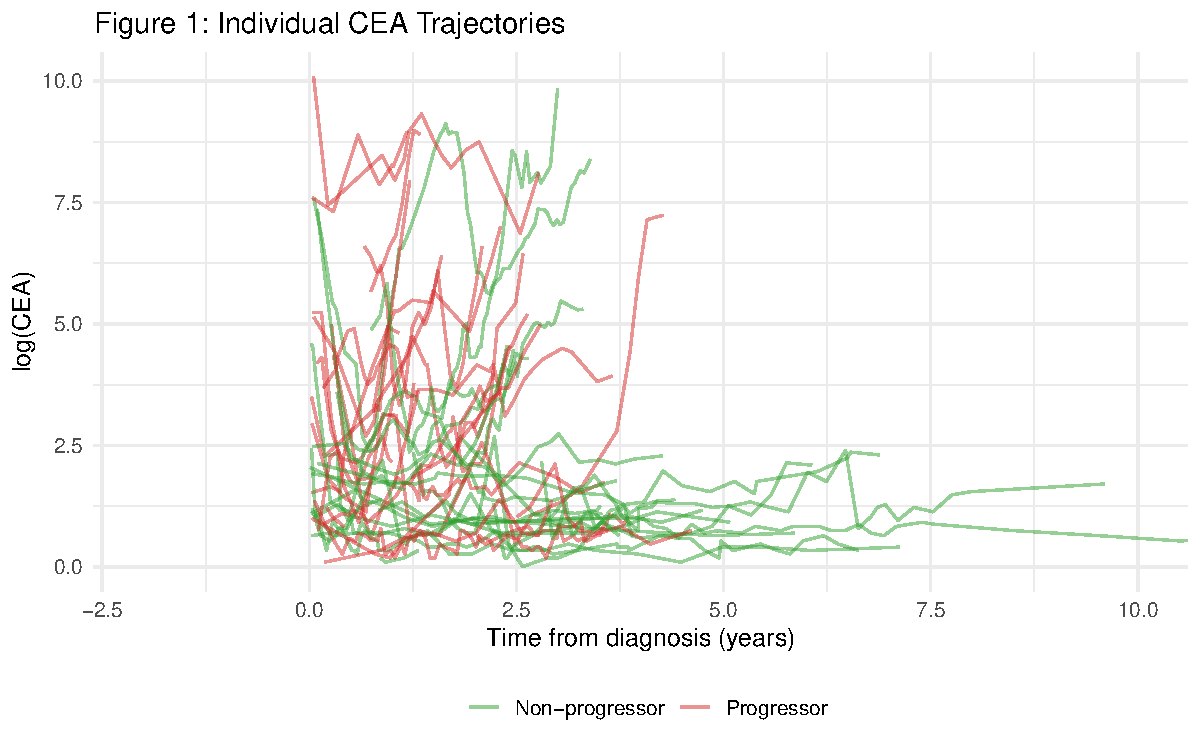
\includegraphics[width=0.65\textwidth]{fig1_cea_trajectories.pdf}
\caption{Individual CEA trajectories for 25 progressors (red) and 25 non-progressors (green), plotted on the log scale against time from diagnosis. Progressors tend to exhibit higher and rising CEA levels.}
\label{fig:trajectories}
\end{figure}

\section{Statistical Methods}

\subsection*{Model~0: Clinical-Only GLMM}

The baseline model was a generalized linear mixed model with a random patient intercept:
\[
\text{logit}\,P(Y_{ij} = 1 \mid \mathbf{X}_{ij}) = \mathbf{X}_{ij}^\top \boldsymbol{\beta} + b_i, \quad b_i \sim N(0, \sigma^2),
\]
where $i$ indexes patients and $j$ indexes landmarks within patient. Covariates included time since diagnosis (years), active treatment type, age, sex, stage, MSI status, and prior medication status. The random intercept accounts for within-patient correlation across repeated landmarks. Estimation used Laplace approximation (\texttt{glmer}, \texttt{nAGQ = 1}) with the BOBYQA optimizer.

\subsection*{Model~A: Clinical + CEA Trajectory GLMM}

Model~A extends Model~0 by adding three CEA trajectory features: $\log(\text{CEA})_\text{current}$, CEA slope (90d), and CEA CV. The same random-effects structure and estimation procedure were used. Models~0 and~A were fitted on the same complete-case subset to ensure a fair comparison.

\subsection*{Model~B: LASSO with Genomic Covariates}

Model~B further augments the covariate set with TMB and binary indicators for the 10 most recurrently mutated CRC genes. An $L_1$-penalized logistic regression (\texttt{cv.glmnet}, \texttt{alpha = 1}, \texttt{family = "binomial"}) was applied with patient-level 5-fold cross-validation to prevent within-patient information leakage during hyperparameter tuning. The penalty parameter $\lambda_\text{min}$ was selected to minimize cross-validated deviance.

\subsection*{Model Evaluation}

Discrimination was assessed via the area under the receiver operating characteristic curve (AUC), computed on one-landmark-per-patient test subsets (first eligible landmark) to ensure patient independence. Calibration was assessed using the calibration slope on the logit scale: $\text{logit}\,P(Y=1) = \alpha + \beta \cdot \text{logit}(\hat{p})$, where $\beta = 1$ indicates perfect calibration, $\beta < 1$ overconfidence, and $\beta > 1$ underconfidence. The Brier score was also reported. The DeLong test was used for paired AUC comparison (Model~0 vs.~A on the shared subset; Model~A vs.~B on the shared genomic subset).

Data were split 70/30 at the patient level (seed = 629), yielding 2,765 training patients (48,278 landmarks) and 1,185 test patients (19,994 landmarks).

\subsection*{Conformal Prediction Sets}

Split-conformal prediction was applied to construct distribution-free prediction sets for the binary outcome at significance level $\alpha = 0.10$ (target coverage $\geq 90\%$). The training set was further split into a proper training set (50\% of the full data) and a calibration set (20\%). To satisfy the exchangeability assumption of conformal inference, one landmark per patient was used in the calibration set (first eligible landmark, $n = 786$). The conformal base model was a standard GLM (without random effects) fitted on the proper training set. For each calibration observation, the nonconformity score was $s_i = 1 - \hat{p}(Y_i \mid X_i)$. The conformal quantile $\hat{q}$ was computed as the $\lceil(1 - \alpha)(n_\text{cal} + 1)\rceil / n_\text{cal}$ quantile of the calibration scores. A label $y \in \{0, 1\}$ was included in the prediction set if its nonconformity score did not exceed~$\hat{q}$.

\section{Results and Discussion}

\subsection*{CEA Trajectory as an Independent Predictor (Model~0 vs.\ Model~A)}

Table~\ref{tab:or} presents odds ratios from Model~A. The three CEA trajectory features were all statistically significant. CEA slope (90d) had the largest effect (OR $\approx 10^9$ per unit change in log-CEA per day), reflecting the very small scale of daily slope values; a clinically meaningful increase of 0.01 log-CEA/day corresponds to OR~$\approx 1.26$. Current $\log(\text{CEA})$ had OR~$= 1.33$ per unit, and CEA~CV was modestly protective (OR~$= 0.84$), likely reflecting that high variability in the absence of a rising trend is not adverse.

Among clinical covariates, Stage~IV was the strongest predictor (OR~$= 5.73$), consistent with the known prognostic importance of metastatic disease. MSI-H status was associated with lower predicted progression risk (OR~$= 0.19$), aligning with evidence that MSI-H CRC often has a more favorable disease course. Active immunotherapy was also associated with lower predicted risk (OR~$= 0.52$), while prior medication exposure was associated with higher predicted risk (OR~$= 2.27$), likely reflecting more treatment-refractory disease.

\begin{table}[H]
\centering
\caption{Odds Ratios from Model~A (Clinical + CEA Trajectory GLMM)}
\label{tab:or}
\small
\begin{tabular}{lrrl}
\toprule
Variable & OR & 95\% CI & $p$-value \\
\midrule
$\log(\text{CEA})$ current & 1.33 & 1.29--1.37 & $< 10^{-16}$ \\
CEA slope (90d) & $1.12 \times 10^9$ & $1.01 \times 10^8$--$1.24 \times 10^{10}$ & $< 10^{-16}$ \\
CEA CV & 0.84 & 0.75--0.95 & 0.002 \\
Time since dx (yr) & 1.32 & 1.30--1.35 & $< 10^{-16}$ \\
Chemo (vs.\ none) & 0.85 & 0.79--0.91 & $1.8 \times 10^{-5}$ \\
Immunotherapy (vs.\ none) & 0.52 & 0.38--0.72 & $5.5 \times 10^{-5}$ \\
Age (per year) & 0.99 & 0.98--1.00 & $5.1 \times 10^{-5}$ \\
Stage IV & 5.73 & 4.65--7.07 & $< 10^{-16}$ \\
MSI-H & 0.19 & 0.12--0.31 & $3.5 \times 10^{-8}$ \\
Prior med (Yes vs.\ No) & 2.27 & 1.76--2.94 & $5.9 \times 10^{-8}$ \\
\bottomrule
\end{tabular}
\end{table}

The primary comparison between Model~0 (AUC = 0.647) and Model~A (AUC = 0.703) showed a highly significant improvement (DeLong $p = 3.61 \times 10^{-10}$), confirming that CEA trajectory features carry substantial incremental predictive value beyond clinical covariates alone. Figure~\ref{fig:roc} displays the ROC curves for this comparison.

\begin{figure}[H]
\centering
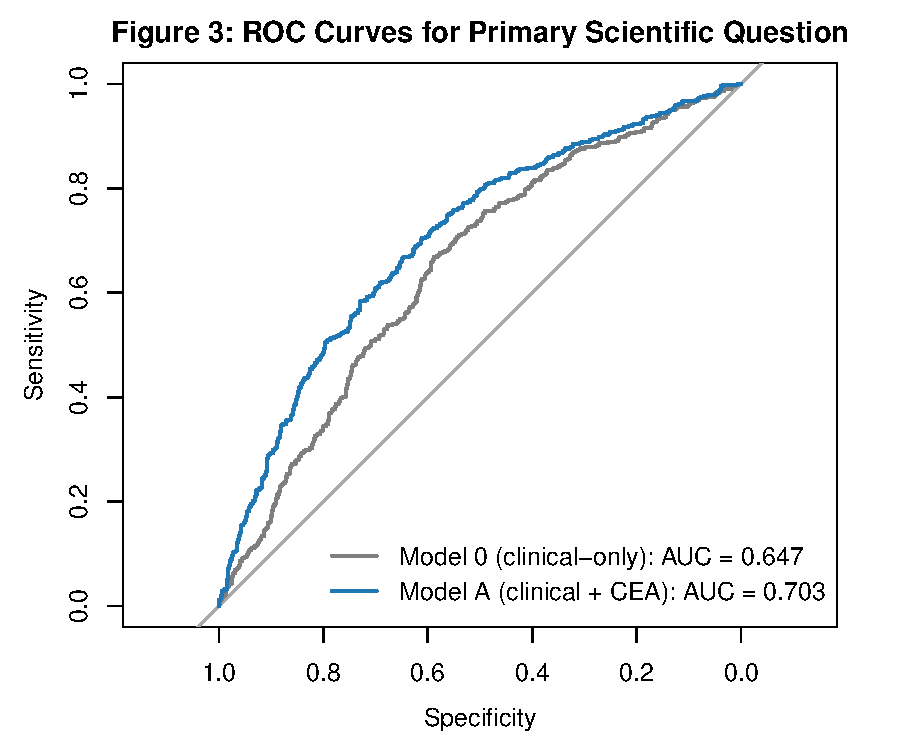
\includegraphics[width=0.65\textwidth]{fig3_roc_curves.pdf}
\caption{ROC curves for Model~0 (clinical-only) and Model~A (clinical + CEA trajectory) on the test set (1 per patient). Adding CEA trajectory features significantly improves discrimination.}
\label{fig:roc}
\end{figure}

\subsection*{Genomic Extension (Model~B)}

The LASSO model retained all 25 candidate features at $\lambda_\text{min} = 0.001$. CEA slope (coefficient = 23.1) and $\log(\text{CEA})$ (0.42) remained the dominant predictors. Among gene-level features, \textit{KRAS} (0.30), \textit{PIK3CA} (0.18), \textit{TP53} (0.16), \textit{SMAD4} (0.15), and \textit{SOX9} (0.17) carried adverse coefficients, while \textit{TCF7L2} ($-0.14$) was modestly protective. TMB had a near-zero coefficient ($-0.003$).

Despite the inclusion of genomic covariates, Model~B achieved AUC~$= 0.7033$ versus $0.7030$ for Model~A on the shared genomic subset of 1{,}180 test patients (DeLong $p = 0.977$). The two values round to the same three-decimal AUC, but they are not literally identical at higher precision; the rounded equality reflects three substantive features of the problem rather than a coding bug. We verified this directly: the Spearman rank correlation between the two models' predicted probabilities on the shared subset is only 0.80, so Models~A and~B do reorder individual patients --- but those reorderings cancel out in aggregate discrimination. (i)~\emph{Dominant signal.} The CEA-trajectory features---especially the 90-day slope and current $\log(\text{CEA})$---carry the overwhelming share of the discriminative information. In the LASSO fit, the CEA-slope coefficient (23.1) and $\log(\text{CEA})$ coefficient (0.42) are orders of magnitude larger than any gene indicator (all $|\hat{\beta}| \leq 0.30$), so the induced risk ranking of test patients changes only marginally when genes are added. (ii)~\emph{Ranking-invariance of AUC.} AUC depends only on the order of predicted risks, not their magnitudes. The two models do disagree on individual patient ranks (Spearman~$\rho = 0.80$ between $\hat{p}_A$ and $\hat{p}_B$), so adding genomic covariates is not a no-op at the patient level --- but the rank changes are roughly evenly distributed between progressors and non-progressors, so the gains and losses on individual progressor / non-progressor pairs almost exactly cancel in the aggregate concordance statistic. (iii)~\emph{Correlation between genomic and clinical/trajectory predictors.} Key mutations (\textit{TP53}, \textit{KRAS}, \textit{SMAD4}) are correlated with stage and with CEA level, so much of their marginal signal is already absorbed by the clinical + CEA block. Consistent with this, Model~B \emph{does} show a modest calibration-slope improvement (0.637 vs.\ 0.515), indicating that genomic covariates sharpen the probability magnitudes even when they do not change the ranking. This comparison should still be interpreted cautiously because Model~A and Model~B differ both in feature set and in modeling framework (GLMM vs.\ LASSO logistic regression without a patient random intercept).

\subsection*{Calibration}

Calibration slopes on the logit scale were 0.408 (Model~0), 0.515 (Model~A), and 0.637 (Model~B), all substantially below~1 (Table~\ref{tab:comparison}). This indicates systematic overconfidence: model-predicted probabilities are too extreme, with high-risk predictions exceeding observed progression rates and low-risk predictions underestimating them. The overconfidence is partially attributable to fixed-effects-only prediction (ignoring patient-specific BLUPs from the random intercept) and the high within-patient correlation structure. Platt scaling or isotonic recalibration on a held-out set would likely improve calibration. Figure~\ref{fig:cal} shows the calibration plot for Model~A.

\begin{figure}[H]
\centering
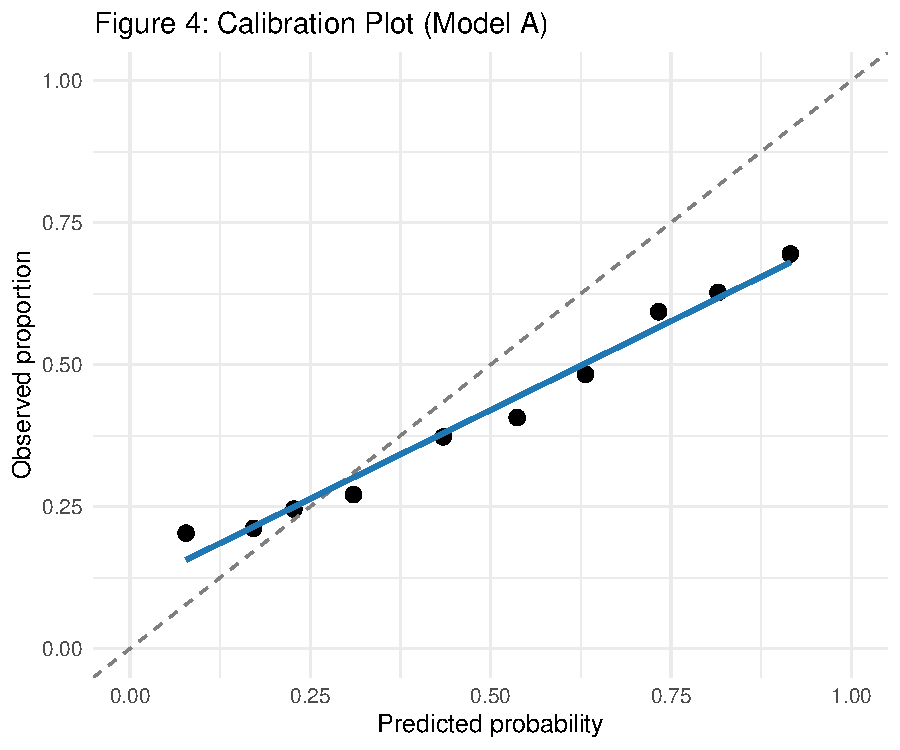
\includegraphics[width=0.55\textwidth]{fig4_calibration.pdf}
\caption{Calibration plot for Model~A on the test set. Points represent deciles of predicted probability. The blue line is a linear fit; the dashed line represents perfect calibration. Model predictions are overconfident (calibration slope = 0.515).}
\label{fig:cal}
\end{figure}

\subsection*{Model Comparison}

Table~\ref{tab:comparison} summarizes discrimination, calibration, and Brier score across all three models.

\begin{table}[H]
\centering
\caption{Model Comparison on Test Set (1 per patient)}
\label{tab:comparison}
\begin{tabular}{llccc}
\toprule
Model & Eval.\ subset & AUC (95\% CI) & Brier Score & Cal.\ Slope \\
\midrule
0: GLMM (clin-only) & clin + CEA CC & 0.647 (0.616--0.679) & 0.2480 & 0.408 \\
A: GLMM (clin + CEA) & clin + CEA CC & 0.703 (0.673--0.733) & 0.2288 & 0.515 \\
B: LASSO (genomic) & genomic CC & 0.703 (0.673--0.734) & 0.2323 & 0.637 \\
\bottomrule
\end{tabular}
\end{table}

The key finding is that CEA trajectory features provide a statistically significant and clinically meaningful improvement in discrimination ($\Delta$AUC = 0.056, $p = 3.61 \times 10^{-10}$). By contrast, the genomic LASSO extension did not show evidence of improved discrimination over Model~A on the shared genomic subset ($\Delta$AUC = 0.000, $p = 0.977$).

\subsection*{Conformal Prediction Sets}

The split-conformal procedure achieved an empirical coverage of 90.1\% on the test set (target $\geq 90\%$), confirming the finite-sample validity guarantee. The conformal quantile was $\hat{q} = 0.718$. Among 1,180 test patients (1 per patient), 34.7\% received singleton prediction sets (a definitive classification into either $\{0\}$ or $\{1\}$), while the remaining 65.3\% received the ambiguous set $\{0, 1\}$, indicating insufficient model certainty to distinguish between progression and non-progression at the 90\% confidence level.

The singleton fraction by predicted risk decile is U-shaped (Supplementary Figure~S2): patients in the lowest and highest risk deciles receive singleton predictions nearly 100\% of the time, while those in intermediate deciles receive almost exclusively ambiguous sets. This aligns with theoretical expectations---the model is most informative for patients whose predicted probability is far from 0.5. Singleton fractions also differ by true outcome: 46.6\% among progressors versus 26.5\% among non-progressors, reflecting the model's asymmetric certainty.

\section{Discussion}

These results support the hypothesis that longitudinal CEA trajectory features---specifically the 90-day slope and current $\log(\text{CEA})$---are strong independent predictors of short-term disease progression in CRC, providing significant incremental value beyond standard clinical variables (AUC 0.647 $\to$ 0.703, $p < 10^{-9}$). The conformal prediction framework provides distribution-free uncertainty quantification, achieving 90.1\% coverage with a 34.7\% singleton rate.

Several limitations warrant consideration. First, calibration slopes of 0.41--0.64 indicate systematic overconfidence in all models. This is partly attributable to the use of population-level fixed-effect predictions without patient-specific BLUPs from the random intercept; recalibration via Platt scaling should be explored. Second, the 90-day slope requirement excludes 14.9\% of patients, biasing the cohort toward those with denser CEA monitoring---likely patients under more active surveillance, who may differ systematically from the excluded patients. Third, timeline variables in MSK-CHORD are recorded only at the day level. Consequently, same-day CEA, treatment, and imaging events cannot be temporally ordered within a day, so the treatment feature should be interpreted as treatment status recorded on or before the landmark day rather than a precisely pre-landmark exposure. Fourth, the LASSO model does not account for within-patient correlation (unlike the GLMM), so its comparison with Model~A is not on strictly equal methodological footing. Fifth, the MSK-CHORD cohort represents a tertiary-referral population, and generalizability to community oncology settings is uncertain.

Future work should include: (1)~Platt scaling or isotonic recalibration to address the overconfidence issue; (2)~a joint longitudinal-survival model that simultaneously models the CEA trajectory process and the progression outcome; (3)~a competing-risks sensitivity analysis that explicitly codes death within $(t, t + 180]$ as a positive event (or uses a cause-specific hazards framework) rather than excluding such landmarks; (4)~external validation on an independent CRC cohort; and (5)~exploration of additional biomarker trajectories (e.g., CA~19-9) and imaging-derived features.

\section*{Reproducibility}

All code, the analytic pipeline, and this report's source are tracked in the project repository at \url{https://github.com/yananf8899/Biostat629}. The complete analysis is driven by a single script, \texttt{project2\_analysis.R}, executed with R~4.3.0 against the MSK-CHORD~2024 release downloaded from cBioPortal under controlled access. Random seeds are fixed (\texttt{set.seed(629)}) for the train/test split, the cross-validation folds, and the conformal calibration split, so all reported numbers regenerate exactly. Package versions used in the most recent run are recorded in \texttt{sessionInfo.txt} alongside the script. A \texttt{README.md} at the repository root documents the directory layout, data-access steps, and the single command needed to reproduce every figure, table, and number cited in this report.

\appendix
\section*{Supplementary Materials}

\begin{table}[H]
\centering
\caption{Supplementary Table~S1. Analytic Variables: Definitions, Original Names, and Source Files}
\label{tab:variables}
\small
\begin{tabular}{llll}
\toprule
Variable & Type & Source File & Coding \\
\midrule
Progression & Binary & \texttt{data\_timeline\_progression} & Y/N within 180 days \\
$\log(\text{CEA})$ & Cont. & \texttt{data\_timeline\_cea\_labs} & $\log(\text{RESULT} + 0.1)$ \\
CEA slope (90d) & Cont. & Derived & OLS slope over $[t-90, t]$ \\
CEA CV & Cont. & Derived & SD/mean of last 3 values \\
Age & Cont. & \texttt{data\_clinical\_patient} & Years \\
Sex & Binary & \texttt{data\_clinical\_patient} & Male vs.\ Female (ref) \\
Stage & Binary & \texttt{data\_clinical\_patient} & IV vs.\ I--III (ref) \\
MSI status & Binary & \texttt{data\_clinical\_sample} & MSI-H vs.\ MSS (ref) \\
Treatment & Cat. & \texttt{data\_timeline\_treatment} & none/chemo/targeted/immuno/other \\
Prior med & Cat. & \texttt{data\_clinical\_patient} & No (ref)/Yes/Unknown \\
TMB & Cont. & \texttt{data\_clinical\_sample} & Non-synonymous count \\
Gene$_j$ ($\times 10$) & Binary & \texttt{data\_mutations} & $\geq 1$ mutation $= 1$ \\
\bottomrule
\end{tabular}
\end{table}

\begin{figure}[H]
\centering
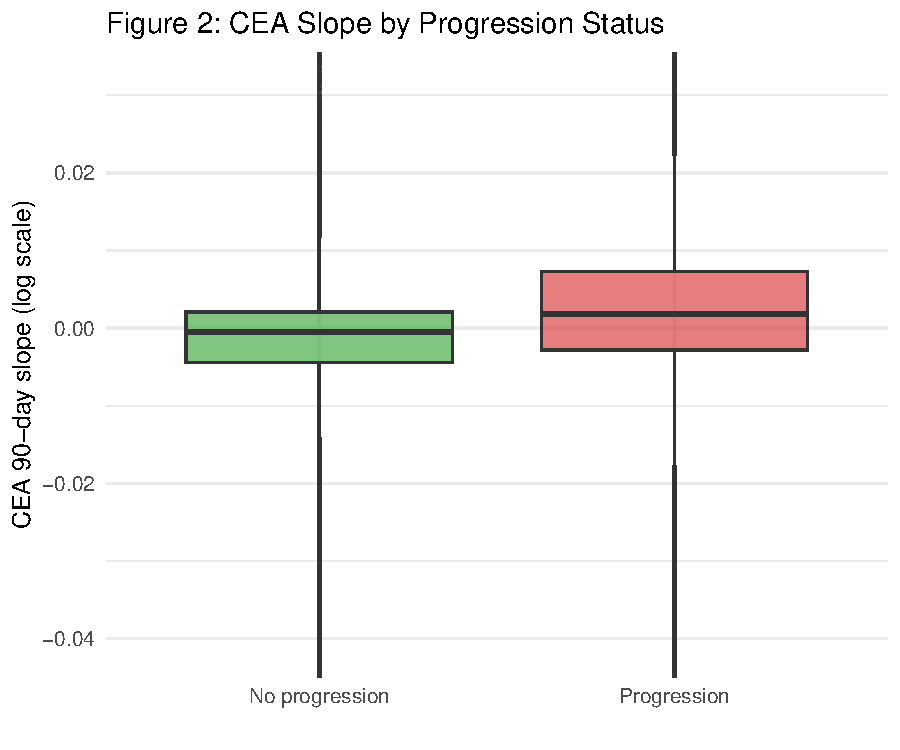
\includegraphics[width=0.55\textwidth]{fig2_cea_slope_boxplot.pdf}
\caption{Supplementary Figure~S1. Distribution of 90-day CEA slope by progression status. The progression group has a higher median slope and a wider interquartile range; whiskers are clipped at the 1st and 99th percentiles.}
\label{fig:slope}
\end{figure}

\begin{figure}[H]
\centering
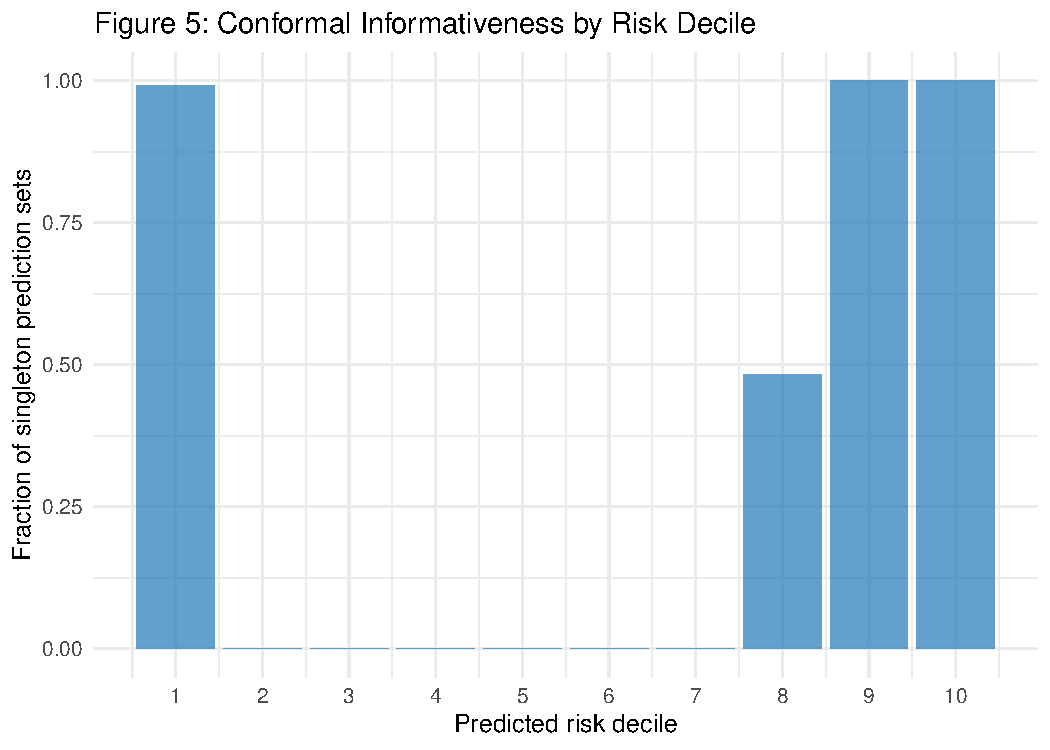
\includegraphics[width=0.65\textwidth]{fig5_conformal_singletons.pdf}
\caption{Supplementary Figure~S2. Fraction of singleton conformal prediction sets by predicted risk decile on the test set. The U-shaped pattern indicates model confidence at the extremes of risk and uncertainty in the middle.}
\label{fig:conformal}
\end{figure}

\end{document}
